

\paragraph{} In this chapter we shall introduce and detail a prototype implementation of a modular, SGX-protected \textit{reference monitor} --- \textsc{Citadel}. First we motivate its necessity and discuss the challenges faced. Then, the three-part architecture will be explained, relating various design decisions to the DIFC model it provides. A discussion about the architecture's performance and effectiveness is provided in §~\ref{sec:eval}.

\section{Motivation}
\paragraph{} Since its introduction in a 1972 report from Anderson,~\cite{reference-monitor} the reference monitor concept has time and again proved to be a reliable workhorse for a plethora of security models. It does not refer to any exact policy, nor limit itself to any particular implementation --- it's abstractness is one of its greatest strengths, reserving any judgement about what policy is \textit{appropriate} in a particular setting.~\cite{irvine-rm}

\paragraph{Fundamental Properties of a Reference Monitor}

\begin{itemize}
    \item \textit{Always invoked.} Every access to the system must be mediated to guarantee that adversaries are unable to bypass the system's security policies.
    \item \textit{Evaluable.} It ``must be small enough to be subject to analysis and tests, the completeness of which can be assured'';~\cite{reference-monitor} to be trustworthy, it must be \textit{auditable}, with, ideally, a restricted TCB.
    \item \textit{Tamper proof.} To ensure that an attacker cannot disable the authorisation mechanisms mandated by the security policy, the integrity of a reference monitor cannot be in question.
\end{itemize}

\paragraph{} No computer system is ever completely secure, and Linux is no exception. Having grown by 1.7 million lines of code (LoC) in the past year alone, to stand at 27.8 million LoC in total,\footnote{\url{https://www.theregister.com/2020/01/06/linux\_2020\_kernel\_systemd\_code/}} bugs are inevitable --- almost 2000 have been reported in the past year,\footnote{\url{https://bugzilla.kernel.org/}} and 662 \textit{severe} bugs are still outstanding.\footnote{\url{https://www.cvedetails.com/product/47/Linux-Linux-Kernel.html}} In this context we must question whether Linux alone can provide a reference monitor implementation the guarantees it requires,~\cite{Lipp2018MeltdownRK, 10.5555/2831143.2831164} thus motivating the use of SGX.

\paragraph{} Applying SGX to this problem brings two attractive benefits;
\begin{itemize}
    \item The system's IFC policy can be evaluable both during offline analysis and online using \textit{attestation}, helping other enclaves' confidence in the underlying system.
    \item SGX's hardware protections are very capable at defending a reference monitor's state, even if adversaries have ring-0 privilege or in the presence of a kernel bug.
\end{itemize}

\section{Challenges}

\begin{figure}[]
    \centering
    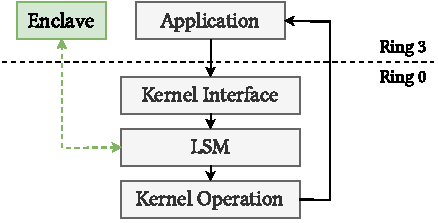
\includegraphics[width=0.48\linewidth]{figures/SGX-EnclaveIntegration.pdf}
    \caption{Abstract \textit{syscall} control flow route. Grey components show the natural Linux design. Green additions highlight the externalised enclave LSM component.}
    \vspace{5mm}
    \label{fig:sgx-abstract-integration}
\end{figure}

\paragraph{} The natural location for a reference monitor is embedded directly in the kernel, in the path of \textit{syscalls'} control flows. \textit{CamFlow} does exactly this using the LSM framework, silently tagging processes and other entities as they are encountered by the kernel, additionally providing an external LSM-interface for any active changes. An SGX enclave is incompatible with this workflow however (§~\ref{sec:sgx-no-kernel-mode}), as it cannot execute alongside kernel code. Thus a major, unavoidable design decision is that the reference monitor must be distributed across rings 0 and 3 --- an enclave \textit{policy} component, and an LSM for \textit{enforcement}.

\paragraph{} The disruption this change causes could severely impact performance; Figure~\ref{fig:sgx-abstract-integration} highlights the significant change to overall control flow. Most notably, externalising part of the LSM to an enclave forces, in the worst case, an additional pair of context switches for each \textit{syscall}.

\paragraph{} Given a ring-3 component is unavoidable, the question becomes how to minimise the overhead caused by its integration, all while maintaining \textit{safety} (every operation must be mediated). This problem is reminiscent of the ones that inspired the development of \textit{exokernels}~\cite{10.1145/224056.224076} --- both the drawbacks and opportunities of those approaches apply here.~\cite{10.1145/269005.266644} \textcolor{red}{More detail about why.}

\paragraph{} Two architectures, as illustrated in Figure~\ref{fig:sgx-integration}, were initially considered. 

\begin{enumerate}
    \item An \textit{isolated} extension of the LSM. Only the security implementation communicates with the \textit{policy} enclave, acting as a na\"{i}ve reimplementation of a fully self-contained LSM, and using an additional kernel module as an I/O relay.
    \item An \textit{integrated} userspace service, through which permission is \textit{requested} ahead of time and decisions stored in the LSM before being needed. Back flow of information is facilitated asynchronously, but an additional kernel relay is not required.
\end{enumerate}



\begin{figure}[]
    \centering
    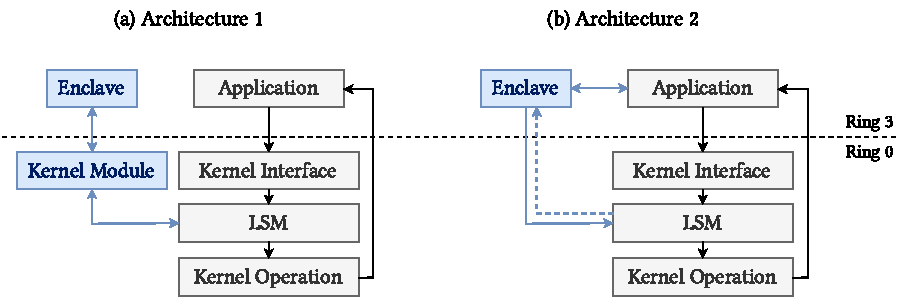
\includegraphics[width=0.98\linewidth]{figures/SGX-EnclaveIntegration-Design}
    \caption{}
    \vspace{2mm}
    \label{fig:sgx-integration}
    \vspace{5mm}
\end{figure}

\paragraph{}\textit{Architecture 1} can be implemented without changing the base IFC model presented in §~\ref{sec:ifc-modelling}, easing potential concerns regarding correctness and safety. However it adds significant overhead to the critical sections~\cite{Dubois1988SynchronizationCA} of core LSM functions, in most cases while the kernel holds locks for various objects being accessed.

\paragraph{} \textit{Architecture 2} is more flexible, requiring all negotiation be conducted ahead of time, and importantly, without leaving userspace: any overhead only impacts the application, leaving the kernel's critical sections to execute with minimal interference. A notable downside, however, is that the system's security model will need to be extended to accommodate the fact that \textit{policy decisions and enforcement are no longer one and the same}.

\paragraph{} Preliminary experiments showed that the performance of the two architectures were similar in light workloads, but \textit{Architecture 1} degrades significantly in the presence of any resource contention. Additionally, as will be explained in §~0.0, the dependence on a kernel module conflicts with the desired constrained TCB of the system. For these reasons \textit{Architecture 2} forms the basis of the prototype.

\paragraph{} An additional challenge is one of incomplete information --- an enclave will not be privy to internal kernel datastructures such as \texttt{task\_struct}, which will store the taint and capabilities of processes. A potential solution would be to implement a request---response model via a custom kernel interface for any queries, though the performance impact would be severe, requiring additional context switches. The approach adopted instead (§~0.0) uses inference based on partial information an enclave has. Any solution must be trustworthy and safe, and malicious entities must not be able to exploit any \textit{eventually consistent} components.~\cite{10.1145/1435417.1435432}

\paragraph{} As a final comment, it must be noted that SGX is not without its flaws; §~5.X discusses this and its impact on the project.


% ---------------

\section{The \textsc{Citadel} IFC Model}

\paragraph{} Before work on the final \textsc{Citadel} implementation began, we constructed a formalisation describing the distributed nature of its design. A model helps reason about the safety and correctness of the final system, and provides the notation to properly discuss its features. Our model, which will now be presented, directly extends the one presented in §~\ref{sec:ifc-modelling}.

\subsection{Reservations}

\paragraph{} Previously we had defined the concept of a \textit{safe flow}, $A \rightarrow B$, which underpins the heart of our IFC restrictions. In previous works permission to perform an operation is granted while \textit{implicitly} considering \textit{how} the flow is to take place (\ref{eqn:res-1}). An isolated \textit{enforcement} component does not understand the concept of \textit{flows}, forcing policy decisions to be defined \textit{explicitly}; \textsc{Citadel} uses \textit{reservations} for this purpose (\ref{eqn:res-2}). This distinction is simple but very important when introducing \textit{laziness} and other optimisations between the two halves of the reference monitor.

\begin{equation}\label{eqn:res-1}
    \textit{operation} \rightarrow \boxed{\textit{reference monitor}} \xrightarrow{\;\;\textit{decision}\;\;} \{0,1\}
\end{equation}
\vspace{-3mm}
\begin{equation}\label{eqn:res-2}
    \textit{operation} \rightarrow \boxed{\textit{policy}\; \xrightarrow{\;\;\textit{reservation}\;\;} \;\textit{enforcement}} \xrightarrow{\;\;\textit{decision}\;\;} \{0,1\}
    \vspace{3mm}
\end{equation}


\paragraph{} Let $\Omega$ be the set of all operations mediated by the reference monitor, including, for example, \texttt{file\_read} or \texttt{socket\_open}. Also, let us define $\mathcal{R}$, the set of all \textit{reservations}, as follows.\footnote{Recalling that $\mathcal{T}$ is the set of all tags.}

\newcommand{\powerset}{\raisebox{.15\baselineskip}{\Large\ensuremath{\wp}}}
\vspace{-7mm}
\begin{equation*}
    \mathcal{R} = \mathcal{T} \times \powerset(\Omega)
    \vspace{2mm}
\end{equation*}

\paragraph{} Further, we define a shorthand, $t^{\alpha}$;
\vspace{-3mm}
\begin{equation*}
    r \in \mathcal{R} \;.\; (r = (t, \alpha) = t^{\alpha} \implies t \in \mathcal{T} \; \wedge \; \alpha \subseteq \Omega)
\end{equation*}

\paragraph{} We introduce, for a process $A$, additional state; $A_{r} \subseteq \mathcal{R}$, the set of all reservations it holds. Once a decision has been made, it is important for a reference monitor to be able to change it, revoking access if required. Thus we specify a notion of \textit{validity} with an indicator function, $\mathcal{V}: \mathcal{R} \mapsto \{0,1\}$. A reservation can only be used to obtain access to a resource if it is valid; invalid reservations are discarded.

\subsection{Permissible Operations}
\label{sec:permissible-operations}

\paragraph{Satisfiability} To determine whether an operation may be permitted, the \textit{constraint reservation} representing it is compared against reservations held by the process. As an example, $t^{\{\texttt{file\_read}\}}$ is the constraint for reading a file tagged with $t$.

\paragraph{} A constraint $\tau^{x}$ is said to be satisfied by a reservation $\tau^{y}$ ($\tau^{x} \sprecsim \tau^{y}$) if the tags match, the reservation is valid, and $y$ permits \textit{at least} the required form of access (\ref{eqn:satis-1}). Equations (\ref{eqn:satis-2}) and (\ref{eqn:satis-3}) define set comparison counterparts --- constraint $\tau^{x}$ is satisfied by a set of reservations $y$ ($\tau^{x} \sqin y$), and a set of constraints $\mu$ is satisfied by a set of reservations $\nu$ ($\mu \sqsubseteq \nu$).

\vspace{-5mm}
\begin{align}
    \sigma^{\alpha}, \tau^{\beta} \in \mathcal{R} &\;.\; (\; \sigma^{\alpha} \sprecsim \tau^{\beta} \iff \sigma = \tau \;\wedge\; \alpha \subseteq \beta \;\wedge\; \mathcal{V}(\tau^{\beta}) \;) \label{eqn:satis-1}\\
    \sigma^{\alpha} \in \mathcal{R}, \; x \subseteq \mathcal{R} &\;.\;  (\; \sigma^{\alpha} \sqin x \iff \exists \, \tau^{\beta} \in x \;.\; \sigma^{\alpha} \sprecsim \tau^{\beta} \;) \label{eqn:satis-2}\\
    \mu, \nu \subseteq \mathcal{R} &\;.\;  (\; \mu \sqsubseteq \nu \iff \forall \, \alpha \in \mu \;.\; \alpha \sqin \nu \;) \label{eqn:satis-3}
\end{align}

\paragraph{} From here we define a \textit{permissible operation}, $A \xrightharpoonup{\;\omega\;} t$; process $A$ may perform operations $\omega$ on an entity tagged with $t$. An operation is only permissible if the process holds a reservation explicitly granting permission (\ref{eqn:permissible-op}).
\begin{equation}
    \label{eqn:permissible-op}
    A \xrightharpoonup{\;\omega\;} t \iff (\exists \; t^{\alpha} \in A_r \implies t^{\omega} \sprecsim t^{\alpha})
\end{equation}

\paragraph{} To bridge the gap between permissible flows and operations, a final definition is required; a \textit{specific permissible flow}, $A \,\xmapsto{\;\omega,\tau\;}\, B$, meaning that $A$ may send information to $B$ using operations $\omega$, via entities tagged with $\tau$. Two natural statements fall out from these definitions;

\vspace{-7mm}
\begin{align}
    (\exists\, \omega,\tau \;.\; A \,\xmapsto{\;\omega,\tau\;}\, B) \implies & A \rightarrow B \\
    A \,\xmapsto{\;\omega,\tau\;}\, B \implies & (\exists \,\omega' \;.\; A \xrightharpoonup{\;\omega'\;} \tau \;\land\; \omega \subseteq \omega') \label{eqn:flow-abs-conc-map}
\end{align}

\paragraph{} Together, these define the relationship between an abstract policy space ($A \rightarrow B$, §~\ref{sec:policy-enclave}) and concrete implementation ($A \xrightharpoonup{\;\omega\;} \tau$, §~\ref{sec:enforcement-domain}). As (\ref{eqn:flow-abs-conc-map}) suggests, a policy decision may grant a greater set of permissions than asked for --- e.g. allowing both read and write when only write was explicitly requested.~\cite{flume,Zeldovich2008}

\paragraph{} A handful of small updates are required to make the existing rules consistent with the new: reservations are not transferred when creating a new entity (\ref{eqn:new-creation}), and reservations are not affected by capabilities as they represent a centralised component of the DIFC system. 

\vspace{-5mm}
\begin{equation}
    A \Rightarrow B \implies A_s = B_s \; \wedge \; A_i = B_i \; \wedge \; B_r = \varnothing \label{eqn:new-creation}
\end{equation}


\subsection{Transient Entities}
\label{sec:transient-entities}

\paragraph{} Alongside active and passive entities, we introduce a third type; \textit{transient} entities. These are passive entities that are privately held by an owning active entitiy; they will be used to model Linux functions such as \texttt{pipe()} and unclaimed tainted files.

\paragraph{} To facilitate this, all processes will be assigned a unique tag $p \in \mathcal{T}$, and any files it creates will initially also be tagged with $p$. Using $\mathcal{P}$ as the set of all process identifiers, we define $\mathcal{I}$ as the function returning a process's transient identifier;

\vspace{-5mm}
\begin{equation}
    \mathcal{I}: \mathcal{P} \mapsto \mathcal{T}
\end{equation}

\paragraph{} The modified expression for a \textit{permissible operation} now becomes;

\vspace{-5mm}
\begin{equation}
    A \xrightharpoonup{\;\omega\;} t \iff \mathcal{I}(A) = t \;\lor\; (\exists \; t^{\alpha} \in A_r \implies t^{\omega} \sprecsim t^{\alpha})
\end{equation}

% ---------------
\clearpage
\section{Implementation}

\begin{figure}[]
    \centering
    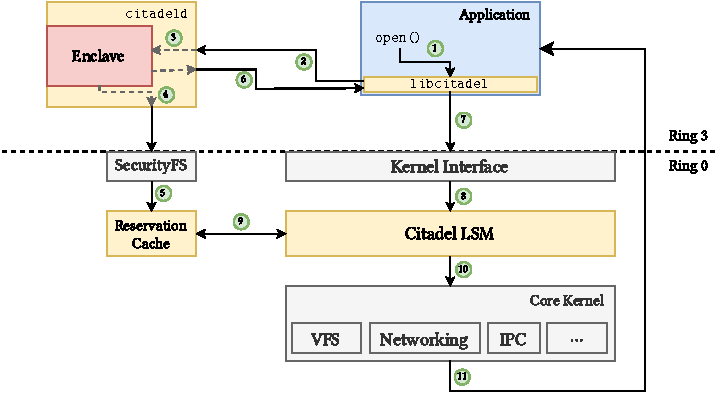
\includegraphics[width=\linewidth]{figures/OverallArchitecture.pdf}
    \caption{High level overview of the \textsc{Citadel} architecture.}
    \vspace{-5mm}
    \label{fig:citadel-overview}
    \vspace{5mm}
\end{figure}

\paragraph{} \textsc{Citadel} consists of three components; an LSM, \texttt{citadeld}, and \texttt{libcitadel}. Each plays an essential, symbiotic role in the operation of the reference monitor. The prototype required in excess of 9,000 lines of C and C++, and extends the Linux kernel build system (§~\ref{sec:build-system}). This section shall present \textsc{Citadel}'s architecture, guided by Figure~\ref{fig:citadel-overview}.

\paragraph{Analogy} The system is well modelled by the \textit{will-call} system used by theatres and the like --- clients (\textit{processes}) reserve tickets (\textit{permission}) to attend a show (\textit{perform an operation}) ahead of time via phone or the internet (\texttt{citadeld}), but only receive their tickets (\textit{reservations}) at the venue (\textit{LSM}) on the day (\textit{at the point of execution}).

\paragraph{} \textsc{Citadel}'s ring-0 components comprise its \textit{enforcement domain} (§~\ref{sec:enforcement-domain}), and \texttt{citadeld} components its \textit{policy domain} (§~\ref{sec:policy-enclave}). The enforcement domain is \textit{policy-agnostic}, implementing an abstract, tagged taint tracking system that exposes decision points to policy influence via reservations. In contrast, policy components need not be aware of the exact enforcement strategy to successfully express their protection schemes. Communication between the two domains is discussed separately in §~\ref{sec:interdomain-comms}.



\subsection{Enforcement}
\label{sec:enforcement-domain}

\begin{figure}[]
    \centering
    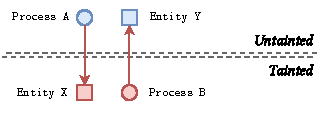
\includegraphics[width=0.55\linewidth]{figures/CitadelTaint.pdf}
    \caption[Accesses across the taint boundary]{Accesses across the taint boundary taint the untainted party.}
    \label{fig:taint-boundary}
\end{figure}

\paragraph{} The \textsc{Citadel} LSM tracks all entities within the Linux system by allocating and attaching a small data structure ($<48$ bytes) to each; it computes and tracks a conservative notion of \textit{taint} for each to ensure \textit{safety}. Tainting in \textsc{Citadel} is dynamic, meaning that entities are only policed if there is a reason. This process is \textit{additive}, only tainting an object if it is involved in a successful operation crossing the taint boundary (Figure~\ref{fig:taint-boundary}); this includes the child process created when a tainted process calls \texttt{fork()}. In additional to automatic propagation, taint for the majority of entities is amendable on request from the policy domain.

\paragraph{} Recalling that entities can either be \textit{active} or \textit{passive}, a variety of metadata is tracked for each.

\begin{enumerate}
    \item[---]\textbf{Active}. The only active entities in Linux are processes --- these require a plethora of markers and flags, including; \textit{taint} and its \textit{reservation list}. The remaining metadata is introduced in §~4.X.
    \item[---] \textbf{Passive}. There are many forms of passive entity, the most prevalent being files and other inode-backed structures. These carry \textit{taint}, an \textit{identifier} (tag), and an \textit{anonymous flag}. Inode tracking is detailed first, with other types of passive entities, such as shared memory, discussed in §~4.X. 
\end{enumerate}

\subsubsection{Identifiers}
\paragraph{} Entities may be tagged with a single identifier; this corresponds to a tag in the IFC model, and are randomly assigned 128-bit numbers. If a security policy wishes to maintain pseudonyms for secrecy and integrity, for example, it may internally, but must convert back to the system tag for enforcement.

\subsubsection{Extended Attributes} 
\paragraph{} An inode-backed entity's taint flag and identifier are copied to \textit{xattrs} attached to it via the VFS. These occupy the \texttt{security.citadel} namespace, and are essential for ensuring that taints and identifiers persist between boots. Certain entities may be \textit{anonymous}, as indicated by their anonymous flag, meaning that their identifier is not present as an \textit{xattr}. This may either be because the entity does not support \textit{xattrs} (such as files created using \texttt{pipe()}) or that the identifier is temporary (§~\ref{sec:entity-creation}).


\subsubsection{Permissions} 
\paragraph{} Tainted processes must hold a valid reservation in their reservation list to perform any operation that may allow data to flow to another entity; the code for this check is attached in Appendix X for reference, but strictly follows the formal rules presented in §~\ref{sec:permissible-operations}. Untainted processes bypass all checks, and thus lie outside the IFC model; the security implications of this are discussed in §~4.X.


\subsubsection{Reservation Cache} 
\paragraph{} When the system's policy domain presents a new reservation to the LSM, it is stored in a structure called the \textit{reservation cache}. Implemented as a red-black tree, it maps a process's identifier to a linked list of its pending reservations. This intermediary storage is necessary as LSMs are event-driven, and thus can only access an entity's state when it is presented for review. Before a permission check is carried out, the LSM ensures that the process's reservation list is up to date by;
\begin{enumerate}
    \item \textit{Installing pending tickets}. All reservations held for the process are moved to its internal reservation list, ready for inspection.
    \item \textit{Disposing of expired entries}. The validity function the LSM uses is time-based. When a reservation is inserted into the reservation cache, it is timestamped with an explicit expiry date --- this lifetime is $15$ seconds by default.  
\end{enumerate}


\subsubsection{Entity Creation}
\label{sec:entity-creation}
\paragraph{} As detailed in §~\ref{sec:transient-entities}, every newly spawned process is privately tagged by the LSM as if it were a passive entity. The purpose of this identifier is not to directly identify the process, but to provide a mechanism for associating any private, passive entities it creates with it. This includes the file descriptors provided by \texttt{pipe()}, and any new files it creates using \texttt{open()}. Every process always has permission to access its transient entities, and external entities can only gain the right to access them if they;
\begin{enumerate}
    \item Are a child processes and request access to their parent, or
    \item The process officially \textit{claims} them via the policy enclave, which gives them an independent tag and removes the entity's status as transient. 
\end{enumerate}


\paragraph{\texttt{fork()}} In Linux, child processes are initially exact clones of their parent, with access to the same state and file descriptors. Thus children of tainted processes are also tainted, but importantly do not assume the same rights as their parents --- open file descriptors will not fucntion without revalidation (§~4.X), and children must request the right to to their parent's transient entities via a special command to use pipes or similar. It is the prerogative of the policy enclave to validate that the security contexts of the parent and child have not diverged. \textcolor{red}{mention leakage through fd state}





\subsection{Policy Components}
\label{sec:policy-enclave}

\paragraph{} The policy counterpart to the LSM's enforcement is contained within \texttt{citadeld}, a userspace service that hosts the core SGX enclave. \texttt{citadeld} is modular, hosting an independent policy module sitting on top of an enforcement translation library (Figure~\ref{fig:policy-enclave}).

\subsubsection{Abstract Security Models}
\paragraph{} The policy module embedded in \texttt{citadeld} is presented with a simple, event-driven interface that abstracts the reality of enforcement away; these policy module are referred to as ASMs. Their implementation is based around a single method, through which their permission is sought when required; \texttt{asm\_handle\_request(3)}.


\paragraph{} The simplest possible ASM is as follows; any operation between or using any entity is deemed permissible. The request parameter, amongst other things, holds the target identifier and set of operations. 

\begin{minted}[fontsize=\footnotesize]{c}
citadel_response_t asm_handle_request (pid_t pid, 
        struct citadel_op_request *request, void *metadata) {
    return CITADEL_OP_APPROVED;
}
\end{minted}

\begin{figure}[]
    \centering
    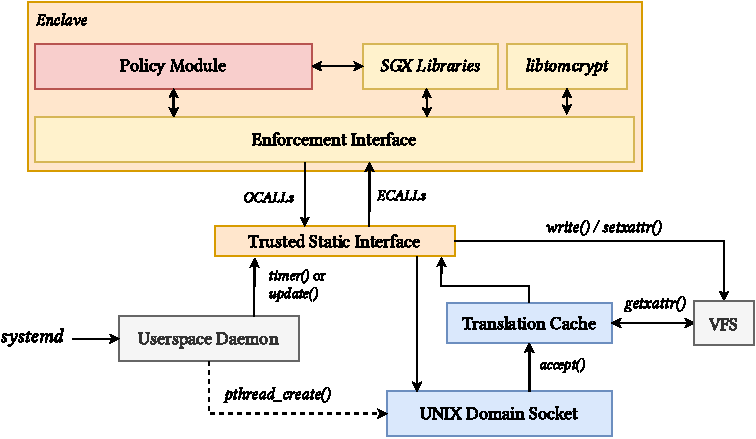
\includegraphics[width=0.9\linewidth]{figures/EnclaveLayout.pdf}
    \caption{Overview of the components inside \texttt{citadeld}.}
    \label{fig:policy-enclave}
\end{figure}

\paragraph{} This can be considered to determine the validity of an operation, $A \xrightharpoonup{\;\omega\;} t$, based on its knowledge of any implicated flows ($A \rightarrow *$).

\paragraph{Operations} Entity operations, $\Omega$, are presented as \texttt{citadel\_operation\_t}, a simple bit mask over the operations \textsc{Citadel} recognises (Appendix X). Similarly, policy decisions are represented using \texttt{citadel\_response\_t}; these may be \textit{approved}, \textit{rejected}, \textit{error}, \textit{invalid}, \textit{granted},\footnote{Approved, and confirming that the process is recognised as the owner of the entity.} and \textit{forged}.\footnote{Discussed in §~4.X.}


\subsubsection{Host Application}
\paragraph{} Before requests (§~4.X) are presented to the resident ASM, various steps need to be taken in preparation. Requests often refer to absolute filepaths, creating a need to retrieve their tags, if they exist --- these requests are served by the security \textit{xattrs} attached to the VFS file. Translation is performed preemptively depending on the operation requested, and to minimise any lookup overhead, results are cached in a \textit{translation cache}. This is implemented using \textit{sparsehash},\footnote{\url{https://github.com/sparsehash/sparsehash}} taking great care to detect and remove stale items.


\subsubsection{Enforcement Interface}
\paragraph{} The policy module is interchangeable, but the enforcement interface acts as the backbone of the enclave. All requests are routed through it as a sanitsation step, detecting forgery or and invalid data, and all information leaving it is formatted and signed\footnote{Encryption is discussed in §~\ref{sec:interdomain-comms}} as appropriate. The process of installing reservations created by the enforcement interface, on behalf of the policy module, is detailed in §~\ref{sec:interdomain-comms}.



% \subsubsection{\texttt{libtomcrypt}}
\subsubsection{Initialisation}
\subsubsection{\texttt{libcitadel}}

\subsection{Interdomain Communication}
\label{sec:interdomain-comms}


\subsection{Additional Security Features}

\subsection{\textsc{Citadel} Build System}
\label{sec:build-system}
